\documentclass{article}

\usepackage{listings}
\usepackage{graphicx}
\usepackage{cite}
\usepackage{url}
\usepackage{listings}
\usepackage[margin=0.5in]{geometry}
\usepackage{color}

%\setmonofont{Consolas} %to be used with XeLaTeX or LuaLaTeX
\definecolor{bluekeywords}{rgb}{0,0,1}
\definecolor{greencomments}{rgb}{0,0.5,0}
\definecolor{redstrings}{rgb}{0.64,0.08,0.08}
\definecolor{xmlcomments}{rgb}{0.5,0.5,0.5}
\definecolor{types}{rgb}{0.17,0.57,0.68}

\usepackage{listings}
\lstset{captionpos=b,
%numbers=left, %Nummerierung
%numberstyle=\tiny, % kleine Zeilennummern
frame=lines, % Oberhalb und unterhalb des Listings ist eine Linie
showspaces=false,
showtabs=false,
breaklines=true,
showstringspaces=false,
breakatwhitespace=true,
escapeinside={(*@}{@*)},
commentstyle=\color{greencomments},
morecomment=[l][\color{greencomments}]{(*},
morekeywords={IF,END_IF,OR,AND,ELSE,THEN},
keywordstyle=\color{bluekeywords},
stringstyle=\color{redstrings},
basicstyle=\ttfamily\small,
}

\title{BRS TwinCAT Description}
\author{M.P.Ross, K.Venkateswara}
\begin{document}
\maketitle
\section{Introduction}
\url{https://github.com/mpross/BRS-Control}
\section{Installation}
\section{Overview}
\section{Hardware}
\section{User Interface}
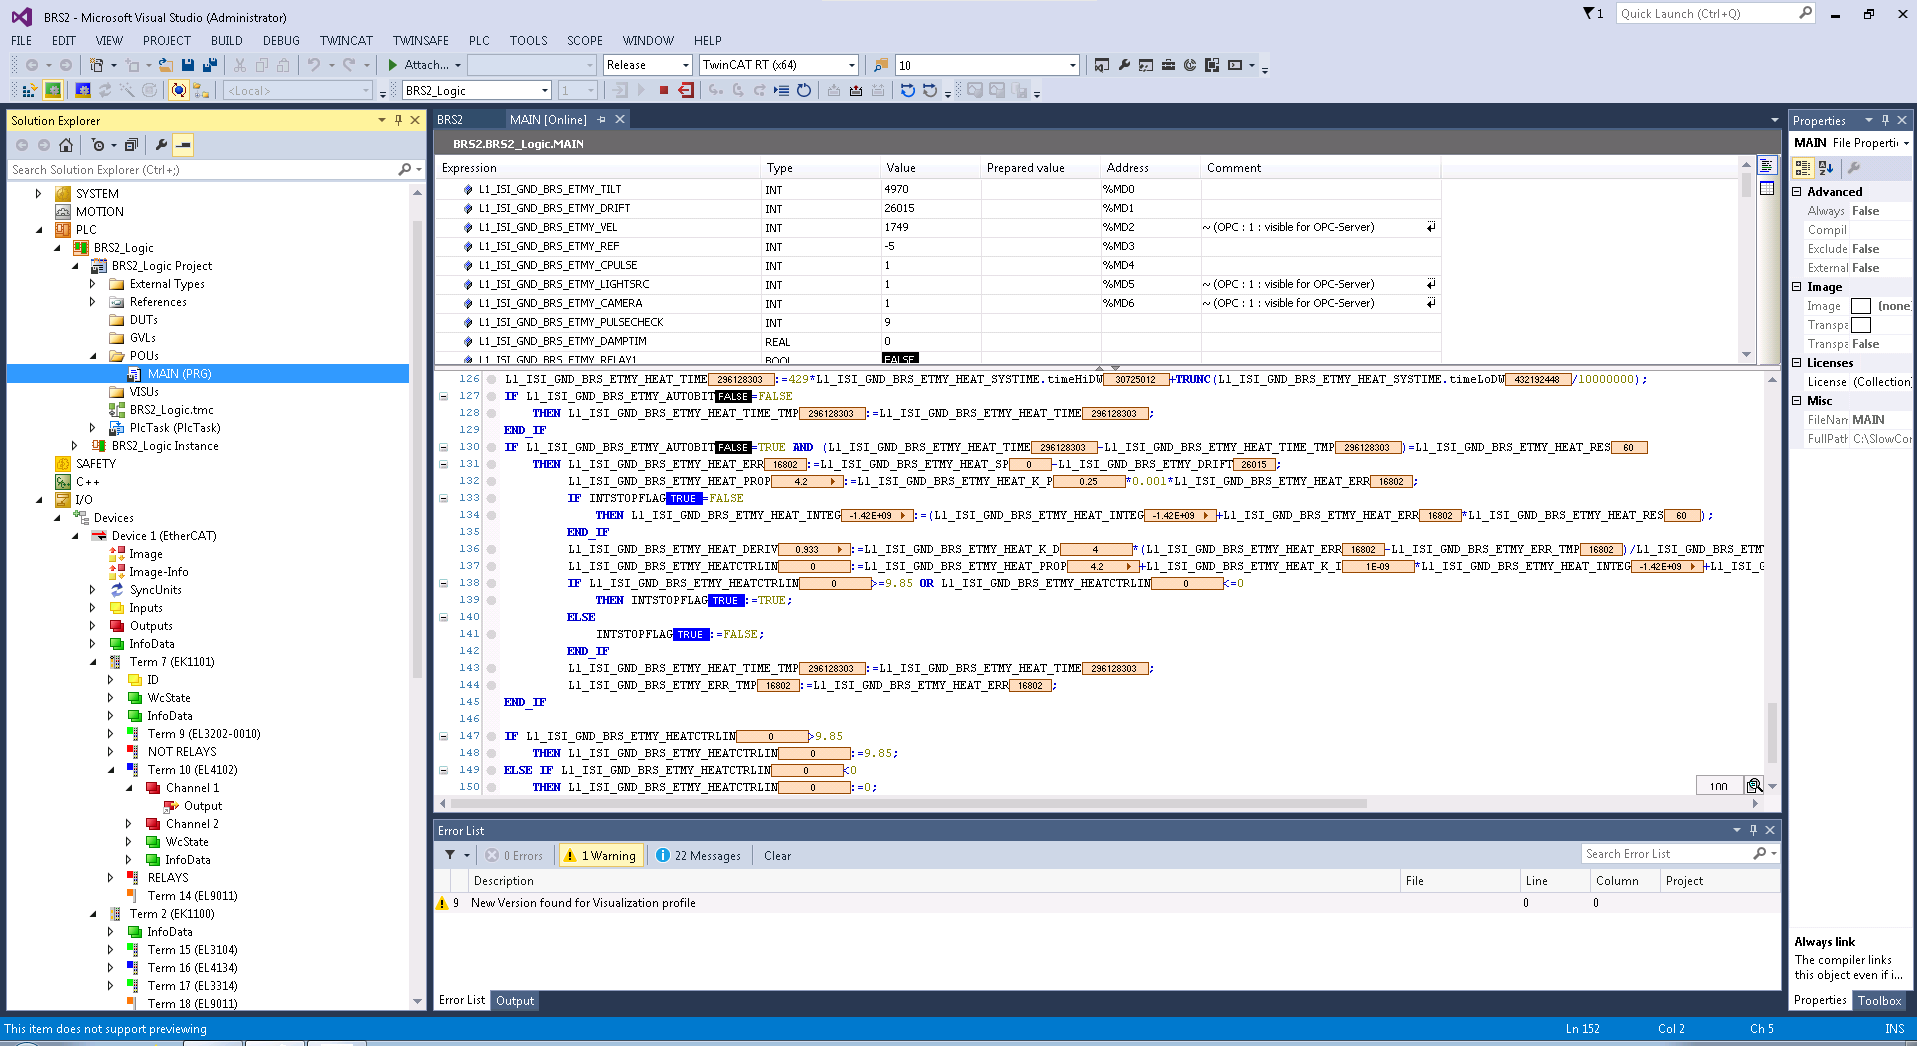
\includegraphics[width=\textwidth]{TwinCATScreen.png}
\section{PLC Variables}
\begin{lstlisting}
VAR
	L1_ISI_GND_BRS_ETMY_TILT AT %MD0: INT;
	L1_ISI_GND_BRS_ETMY_DRIFT AT %MD1: INT;
	L1_ISI_GND_BRS_ETMY_VEL AT %MD2: INT;(*~ (OPC : 1 : visible for OPC-Server) 
										(OPC_PROP[0005] :1: read-only)
										(OPC_PROP[0101] :Sqrt(Velocity): DESC)
										(OPC_PROP[0103] :-500: LOPR)
										(OPC_PROP[0102] :+500: HOPR)
										*)
	L1_ISI_GND_BRS_ETMY_REF AT %MD3: INT;		
	L1_ISI_GND_BRS_ETMY_CPULSE AT %MD4: INT;
	L1_ISI_GND_BRS_ETMY_LIGHTSRC AT %MD5: INT;(*~ (OPC : 1 : visible for OPC-Server)
										(OPC_PROP[0005] :1: read-only)
										(OPC_PROP[0101] :Light Source Status: DESC)
										*)
	L1_ISI_GND_BRS_ETMY_CAMERA AT %MD6: INT;(*~ (OPC : 1 : visible for OPC-Server)
										(OPC_PROP[0005] :1: read-only)
										(OPC_PROP[0101] :Camera Status: DESC)
										*)
	
	L1_ISI_GND_BRS_ETMY_PULSECHECK: INT:=0;
	L1_ISI_GND_BRS_ETMY_DAMPTIM: REAL;
	L1_ISI_GND_BRS_ETMY_RELAY1: BOOL;
	L1_ISI_GND_BRS_ETMY_RELAY2: BOOL;
	L1_ISI_GND_BRS_ETMY_DRIFTBIT: BOOL;(*~ (OPC : 1 : visible for OPC-Server)
										(OPC_PROP[0005] :1: read-only)
										(OPC_PROP[0101] :Drift Status: DESC)
										(OPC_PROP[0106] :GOOD: ONAM)
										(OPC_PROP[0107] :BAD: ZNAM)
										*)
	L1_ISI_GND_BRS_ETMY_MODBIT: BOOL;(*~ (OPC : 1 : visible for OPC-Server)
										(OPC_PROP[0005] :1: read-only)
										(OPC_PROP[0101] :ISI Modules Status: DESC)
										(OPC_PROP[0106] :GOOD: ONAM)
										(OPC_PROP[0107] :BAD: ZNAM)
										*)
	L1_ISI_GND_BRS_ETMY_BOXBIT: BOOL;(*~ (OPC : 1 : visible for OPC-Server)
										(OPC_PROP[0005] :1: read-only)
										(OPC_PROP[0101] :BRS Box Status: DESC)
										(OPC_PROP[0106] :GOOD: ONAM)
										(OPC_PROP[0107] :BAD: ZNAM)
										*)
	L1_ISI_GND_BRS_ETMY_CAPDRIVE: INT;
		
	L1_ISI_GND_BRS_ETMY_TEMPL AT %IW0: INT;(*~ (OPC : 1 : visible for OPC-Server)
										(OPC_PROP[0005] :1: read-only)
										(OPC_PROP[0101] :Tempurature Left: DESC)
										(OPC_PROP[0100] :1/100 C: EGU)
										*)
	L1_ISI_GND_BRS_ETMY_TEMPR AT %IW1: INT;(*~ (OPC : 1 : visible for OPC-Server)
										(OPC_PROP[0005] :1: read-only)
										(OPC_PROP[0101] :Tempurature Right: DESC)
										(OPC_PROP[0100] :1/100 C: EGU)
										*)
	L1_ISI_GND_BRS_ETMY_BOXIN AT %IW2: BOOL;
	L1_ISI_GND_BRS_ETMY_MOD1IN AT %IW3: BOOL;
	L1_ISI_GND_BRS_ETMY_MOD2IN AT %IW4: BOOL;	
	L1_ISI_GND_BRS_ETMY_USER: BOOL:=TRUE;(*~ (OPC : 1 : visible for OPC-Server)
											(OPC_PROP[0005] :3: read/write)
											(OPC_PROP[0101] :User Damping Control: DESC)
											(OPC_PROP[0106] :On: ONAM)
											(OPC_PROP[0107] :Off: ZNAM)
											*)	
	L1_ISI_GND_BRS_ETMY_LOWTHRESHOLD: INT:=800;(*~ (OPC : 1 : visible for OPC-Server)
										(OPC_PROP[0005] :3: read/write)
										(OPC_PROP[0101] :Lower Damping Threshold: DESC)*)
	L1_ISI_GND_BRS_ETMY_HIGHTHRESHOLD: INT:=2000;(*~ (OPC : 1 : visible for OPC-Server)
										(OPC_PROP[0005] :3: read/write)
										(OPC_PROP[0101] :Upper Damping Threshold: DESC)*)
	L1_ISI_GND_BRS_ETMY_DAMPTIMEOUT: REAL:=62500;(*~ (OPC : 1 : visible for OPC-Server)
										(OPC_PROP[0005] :3: read/write)
										(OPC_PROP[0101] :Damping Timeout: DESC)*)
	
	L1_ISI_GND_BRS_ETMY_CAPOUTL AT %QW0: INT;
	L1_ISI_GND_BRS_ETMY_CAPOUTR AT %QW1: INT;
	L1_ISI_GND_BRS_ETMY_AMPBIT AT %QW3: BOOL;(*~ (OPC : 1 : visible for OPC-Server)
											(OPC_PROP[0005] :1: read-only)
											(OPC_PROP[0101] :Amplitude Status: DESC)
											(OPC_PROP[0106] :GOOD: ONAM)
											(OPC_PROP[0107] :BAD: ZNAM)
											*)
	L1_ISI_GND_BRS_ETMY_TILTOUT AT %QW4: INT;
	L1_ISI_GND_BRS_ETMY_DRIFTOUT AT %QW5: INT;
	L1_ISI_GND_BRS_ETMY_REFOUT AT %QW6: INT;
	L1_ISI_GND_BRS_ETMY_DAMPBIT AT %QW7: BOOL;(*~ (OPC : 1 : visible for OPC-Server)
											(OPC_PROP[0005] :1: read-only)
											(OPC_PROP[0101] :Damping Status: DESC)
											(OPC_PROP[0106] :Damping: ONAM)
											(OPC_PROP[0107] :Not Damping: ZNAM)
											*)
	
	L1_ISI_GND_BRS_ETMY_CBIT AT %QW8: BOOL; (*~ (OPC : 1 : visible for OPC-Server)
											(OPC_PROP[0005] :1: read-only)
											(OPC_PROP[0101] :C# Running Status: DESC)
											(OPC_PROP[0106] :GOOD: ONAM)
											(OPC_PROP[0107] :BAD: ZNAM)
											*)
	
	L1_ISI_GND_BRS_ETMY_RELAYL AT %QW9: BOOL;
	L1_ISI_GND_BRS_ETMY_RELAYR AT %QW10: BOOL;
	L1_ISI_GND_BRS_ETMY_NOTRELAYL AT %QW11: BOOL;
	L1_ISI_GND_BRS_ETMY_NOTRELAYR AT %QW12: BOOL;
	L1_ISI_GND_BRS_ETMY_STATUSOUT AT %QW13: INT;
	
END_VAR
\end{lstlisting}
\section{PLC Loop}
\begin{lstlisting}
(*User master switch for damping*)
IF L1_ISI_GND_BRS_ETMY_USER=TRUE
THEN 
	(*If damper is on. 3276 = 1V output*)
	IF L1_ISI_GND_BRS_ETMY_DAMPBIT=TRUE
	THEN
		(*If under lower threshold the damping timer turns on.*)
		IF ABS(L1_ISI_GND_BRS_ETMY_VEL)<L1_ISI_GND_BRS_ETMY_LOWTHRESHOLD
			(*Checks to see if damping timer is off and start Timer.*)
			THEN IF L1_ISI_GND_BRS_ETMY_DAMPTIM <=0
				THEN L1_ISI_GND_BRS_ETMY_DAMPTIM:=1;
					L1_ISI_GND_BRS_ETMY_CAPDRIVE:=L1_ISI_GND_BRS_ETMY_VEL;
				(*Damping timeout check*)
				ELSE IF L1_ISI_GND_BRS_ETMY_DAMPTIM<L1_ISI_GND_BRS_ETMY_DAMPTIMEOUT
					THEN 
					L1_ISI_GND_BRS_ETMY_CAPDRIVE:=L1_ISI_GND_BRS_ETMY_VEL;
					L1_ISI_GND_BRS_ETMY_DAMPTIM:=L1_ISI_GND_BRS_ETMY_DAMPTIM+1;
					(*Damper timeout reset*)
					ELSE
						L1_ISI_GND_BRS_ETMY_DAMPBIT:=FALSE;
						L1_ISI_GND_BRS_ETMY_CAPDRIVE:=0;
						L1_ISI_GND_BRS_ETMY_DAMPTIM:=0;
						L1_ISI_GND_BRS_ETMY_RELAY1:=FALSE;
						L1_ISI_GND_BRS_ETMY_RELAY2:=FALSE;
					END_IF
				END_IF
			(*If above lower threshold continue damping*)
			ELSE
				L1_ISI_GND_BRS_ETMY_RELAY2:=FALSE;
				L1_ISI_GND_BRS_ETMY_CAPOUTL:=L1_ISI_GND_BRS_ETMY_CAPDRIVE;
				L1_ISI_GND_BRS_ETMY_CAPOUTR:=0;
				L1_ISI_GND_BRS_ETMY_DAMPTIM:=0;
				L1_ISI_GND_BRS_ETMY_CAPDRIVE:=L1_ISI_GND_BRS_ETMY_VEL;
			END_IF
			(*If capdrive is positive send to left capacitor, if negative send to right capacitor*)
			IF L1_ISI_GND_BRS_ETMY_CAPDRIVE >= 0
			THEN L1_ISI_GND_BRS_ETMY_RELAY1:=TRUE;
			ELSE L1_ISI_GND_BRS_ETMY_RELAY2:=TRUE;
				L1_ISI_GND_BRS_ETMY_RELAY1:=FALSE;
				L1_ISI_GND_BRS_ETMY_CAPOUTR:=-L1_ISI_GND_BRS_ETMY_CAPDRIVE;
				L1_ISI_GND_BRS_ETMY_CAPOUTL:=0;
			END_IF	
	(*If damper is off*)
	ELSE 
		(*Upper threshold check.*)
		IF ABS(L1_ISI_GND_BRS_ETMY_VEL)>L1_ISI_GND_BRS_ETMY_HIGHTHRESHOLD
		(*Sets damper on.*)
		THEN L1_ISI_GND_BRS_ETMY_DAMPBIT:=TRUE;				
		(*If below upper threshold turn off damping*)
		ELSE 
			 L1_ISI_GND_BRS_ETMY_RELAY1:=TRUE;
			 L1_ISI_GND_BRS_ETMY_RELAY2:=TRUE;
			 IF L1_ISI_GND_BRS_ETMY_VEL=0
				 THEN L1_ISI_GND_BRS_ETMY_CAPDRIVE:=0;
				 ELSE
					L1_ISI_GND_BRS_ETMY_CAPDRIVE:= (L1_ISI_GND_BRS_ETMY_VEL/ABS(L1_ISI_GND_BRS_ETMY_VEL))*(L1_ISI_GND_BRS_ETMY_VEL*L1_ISI_GND_BRS_ETMY_VEL)/20/1000;
					L1_ISI_GND_BRS_ETMY_CAPOUTL:=L1_ISI_GND_BRS_ETMY_CAPDRIVE+1600;
					L1_ISI_GND_BRS_ETMY_CAPOUTR:=-L1_ISI_GND_BRS_ETMY_CAPDRIVE+1600;
			END_IF	
		END_IF
	END_IF	
(*User control check.*)
ELSE L1_ISI_GND_BRS_ETMY_RELAY1:=FALSE;
	L1_ISI_GND_BRS_ETMY_RELAY2:=FALSE;
	L1_ISI_GND_BRS_ETMY_CAPDRIVE:=0;
	L1_ISI_GND_BRS_ETMY_CAPOUTL:=0;
	L1_ISI_GND_BRS_ETMY_CAPOUTR:=0;
	L1_ISI_GND_BRS_ETMY_DAMPBIT:=FALSE;	
	
END_IF
(*Nonlinear amplitude check. Sets amplitude status bit.*)
IF ABS(L1_ISI_GND_BRS_ETMY_TILT)>10000
	THEN L1_ISI_GND_BRS_ETMY_AMPBIT:=FALSE;
ELSE L1_ISI_GND_BRS_ETMY_AMPBIT:=TRUE;
END_IF
(*Drift amplitude check.*)
IF ABS(L1_ISI_GND_BRS_ETMY_DRIFT)>=32000
	THEN L1_ISI_GND_BRS_ETMY_DRIFTBit:=FALSE;
ELSE L1_ISI_GND_BRS_ETMY_DRIFTBit:=TRUE;
END_IF
(*C# code pulse check. Sets C# code status bit.*)
IF L1_ISI_GND_BRS_ETMY_PULSECHECK>=20
	THEN L1_ISI_GND_BRS_ETMY_PULSECHECK:=0;
	IF L1_ISI_GND_BRS_ETMY_CPULSE=1
		THEN L1_ISI_GND_BRS_ETMY_CBIT:=TRUE;
		L1_ISI_GND_BRS_ETMY_CPULSE:=0;		
	ELSE L1_ISI_GND_BRS_ETMY_CBIT:=FALSE;		
	END_IF
END_IF
IF (L1_ISI_GND_BRS_ETMY_CBIT=FALSE) OR (L1_ISI_GND_BRS_ETMY_DRIFTBIT=FALSE) OR (L1_ISI_GND_BRS_ETMY_LIGHTSRC=0) OR (L1_ISI_GND_BRS_ETMY_CAMERA=0) OR (L1_ISI_GND_BRS_ETMY_MODBIT=FALSE) OR (L1_ISI_GND_BRS_ETMY_BOXBIT=FALSE)
	THEN(*Turns damping off if C# code isn't running.*)
		L1_ISI_GND_BRS_ETMY_CAPDRIVE:=0;
		L1_ISI_GND_BRS_ETMY_RELAY1:=FALSE;
		L1_ISI_GND_BRS_ETMY_RELAY2:=FALSE;
		L1_ISI_GND_BRS_ETMY_DAMPBIT:=FALSE;
END_IF
(*Beckhoff status inversion*)
L1_ISI_GND_BRS_ETMY_BOXBIT:=NOT L1_ISI_GND_BRS_ETMY_BOXIN;
L1_ISI_GND_BRS_ETMY_MODBIT:= NOT L1_ISI_GND_BRS_ETMY_MOD1IN OR NOT L1_ISI_GND_BRS_ETMY_MOD2IN;
(*Overview status out construction. If any error flags are raised set status to 0V, else if damping set to 2 V, else set to 5V*)
IF (L1_ISI_GND_BRS_ETMY_CBIT=FALSE) OR (L1_ISI_GND_BRS_ETMY_AMPBIT=FALSE) OR (L1_ISI_GND_BRS_ETMY_DRIFTBIT=FALSE) OR (L1_ISI_GND_BRS_ETMY_LIGHTSRC=0) OR (L1_ISI_GND_BRS_ETMY_CAMERA=0) OR (L1_ISI_GND_BRS_ETMY_MODBIT=FALSE) OR (L1_ISI_GND_BRS_ETMY_BOXBIT=FALSE)
	THEN 
		L1_ISI_GND_BRS_ETMY_STATUSOUT:=0;
ELSE IF L1_ISI_GND_BRS_ETMY_DAMPBIT=TRUE
	THEN L1_ISI_GND_BRS_ETMY_STATUSOUT:=2*3276;
	ELSE
		L1_ISI_GND_BRS_ETMY_STATUSOUT:=5*3276;
	END_IF
END_IF
L1_ISI_GND_BRS_ETMY_PULSECHECK:=L1_ISI_GND_BRS_ETMY_PULSECHECK+1;
(*Relay states set so the capacitors are either passed the damping signal or grounded.*)
L1_ISI_GND_BRS_ETMY_RELAYL:= L1_ISI_GND_BRS_ETMY_RELAY1;
L1_ISI_GND_BRS_ETMY_RELAYR:= L1_ISI_GND_BRS_ETMY_RELAY2;
L1_ISI_GND_BRS_ETMY_NOTRELAYL:= NOT L1_ISI_GND_BRS_ETMY_RELAY1;
L1_ISI_GND_BRS_ETMY_NOTRELAYR:= NOT L1_ISI_GND_BRS_ETMY_RELAY2;
L1_ISI_GND_BRS_ETMY_TILTOUT:=L1_ISI_GND_BRS_ETMY_TILT;
L1_ISI_GND_BRS_ETMY_DRIFTOUT:=L1_ISI_GND_BRS_ETMY_DRIFT;
L1_ISI_GND_BRS_ETMY_REFOUT:=L1_ISI_GND_BRS_ETMY_REF;
\end{lstlisting}
\section{Signal Processing}

\section{Troubleshooting}
\begin{itemize}
\item 
\begin{enumerate}
\item
\end{enumerate}
\end{itemize}
\end{document}